\documentclass[fleqn,10pt]{wlscirep}
\usepackage[utf8]{inputenc}
\usepackage[T1]{fontenc}
\usepackage{placeins}

\title{Mechanics-guided crack-event detection from multiplexed fiber Bragg grating interrogator signals}

\author[a,c]{A.~Uğurveren}
\author[a]{A.~Gros}
\author[a,c]{E.~Nohutcuoğlu}
\author[a,c]{T.~Tekoğlu}
\author[c]{K.~Yüksel}
\author[a]{K.~Chah}
\author[a,b,*]{C.~Caucheteur}

\affil[a]{Electromagnetism and Telecommunication Department, UMONS, Mons, 7000, Belgium}
\affil[b]{WEL Research Institute, Avenue Pasteur, 6, 1300 Wavre, Belgium}
\affil[c]{FISENS, Izmir Institute of Technology, Urla, 35430, Türkiye}
\affil[*]{christophe.caucheteur@umons.ac.be}

%\keywords{fiber Bragg grating, structural health monitoring, crack localization, deep learning, mechanics-informed learning}

\begin{abstract}
Accurate detection of crack-associated events from optical fiber measurements remains a challenge in structural health monitoring. Existing approaches often rely on engineered spectral indicators, dense distributed sensing, or evaluation protocols that do not reflect specimen-level generalization. Here, we study crack-event detection from short peak-aligned responses extracted from multiplexed fiber Bragg grating (FBG) interrogator signals. The proposed framework combines target-channel wavelength statistics, residualized response features, synchronized loading descriptors, and a simple mechanics-consistency filter derived from elastic beam-response expectations. A compact one-dimensional convolutional neural network is trained on ordered response sequences and evaluated under strict leave-one-run-out validation. On glass-fiber composite beams instrumented with embedded FBG arrays and tested under three-point bending, the best reproducible operating point reaches experiment-level precision of 0.833, recall of 0.667, and F1 score of 0.741. The results show that useful crack-related information is present in multiplexed FBG interrogator signals, while also highlighting the importance of dataset alignment, label definition, and run-level evaluation. The proposed framework is a mechanics-guided crack-event detector for multiplexed FBG measurements.
\end{abstract}

\begin{document}

\flushbottom
\maketitle
\thispagestyle{empty}

\section*{Introduction}

Crack detection remains challenging in structural health monitoring (SHM) because damage initiates locally while maintenance decisions are made at the structural scale. Optical fiber sensing, and in particular fiber Bragg grating (FBG) sensing, is used for this purpose because of low weight, immunity to electromagnetic interference, embeddability, and multiplexing capability along a single fiber line \cite{ye2014,yassin2024,golovastikov2025}. These properties have led to the use of FBG strain sensing in civil, aerospace, and composite structures. In composite materials, previous studies have discussed both the use of embedded FBG networks and the challenges associated with sensor integration, protection, and reliability over time \cite{kinet2014,gabardi2023}. Despite progress in strain measurement, translating interrogator data into robust damage-state information at specimen level remains an open problem.

Recent work has explored learning approaches to interpret optical fiber measurements. In FBG systems, machine learning has been used to track crack initiation and growth in metallic structures, combine long gauge measurements with deep learning for damage identification, and process dynamic responses from FBG arrays using dimensionality reduction and convolutional neural network (CNN) \cite{chilelli2019,zhang2020,wang2023}. Other studies have relied on multispectral feature fusion for fatigue crack monitoring or combined FBG sensing with deep learning for damage identification in composite materials \cite{zhao2025,xiong2025}. In parallel, machine learning has been employed to disentangle strain and temperature effects in multiplexed FBG arrays \cite{saha2025} and to infer transverse force from the full reflected spectrum of a uniform FBG under standard interrogation \cite{tocanne2025}.  While these approaches show that learning algorithms can extract information on damage, they typically rely on engineered features, reduced representations, or specimen labels rather than identifying localized damage directly from raw interrogator signals.

More advanced damage-localization strategies based on deep learning have been reported primarily for distributed fiber optic sensing (DFOS). These include deep learning assisted monitoring of spatially distributed cracks and automated crack quantification from distributed strain measurements while accounting for nonlinear effects \cite{liu2023,lu2025}. Related developments in SHM include neural network based crack detection using strain gauges, hybrid approaches to damage localization, and physics informed frameworks driven by data \cite{yoon2022,moreh2025,si2025}. Although these studies show progress in crack interpretation from sensing data, they generally operate on distributed strain fields, dense sensor networks, or image representations. Multiplexed FBG interrogator data instead provide a small number of synchronized channels and a more indirect view of damage. This study therefore focuses on crack-event detection from multiplexed FBG measurements.

This study addresses that gap by analyzing short fixed-length interrogator windows extracted from the multiplexed interrogator output around detected loading responses. The task is to identify crack-associated windows from the target FBG channel and its companion channels under a run-level evaluation protocol that reflects specimen correlation. This problem can also be informed by structural mechanics. Under Euler-Bernoulli beam theory, the surface strain in a slender beam subjected to bending is related to the applied load and the section geometry \cite{ochsner2021}. Deviations between the measured FBG response and this expected elastic behavior provide damage-related context. This observation motivates the mechanics-guided approach used here for crack-event detection from multiplexed FBG signals.

Building on this idea, we combine peak-aligned interrogator responses with synchronized loading information and features derived from an expected healthy structural response. The retained input representation includes target-channel wavelength statistics, residualized response terms, synchronized force and displacement information, and simple first-difference descriptors that preserve local loading dynamics across repeated responses. A compact temporal CNN is then used to classify crack-associated sequences within each measurement run, and a simple physics-consistency filter is applied at the decision stage. This formulation keeps the learning architecture simple while turning limited multiplexed FBG measurements into a structured detection problem that can be evaluated rigorously.

We make three contributions. First, we formulate crack-event detection from short multiplexed FBG interrogator windows under a specimen-aware run-level validation protocol. Second, we show that synchronized mechanics information can be incorporated effectively through loading descriptors and a physics-consistency filter without resorting to an unnecessarily complex architecture. Third, we demonstrate that dataset alignment and merge strategy materially influence final performance under strict leave-one-run-out evaluation.

\section*{Methodology}

\subsection*{FBG inscription and interrogation}

Uniform FBGs were inscribed in single mode optical fibers by the phase mask technique using a NORIA FBG inscription system (NorthLab Photonics) equipped with a 193 nm excimer laser \cite{nieuwland2016}. During inscription, the reflected spectra were monitored in real time with an optical spectrum analyzer. Fibers of approximately 30 cm and 60 cm were prepared according to the specimen dimensions, and sensing fibers containing single, dual, or triple gratings were fabricated for the initial experimental campaign. Each grating had a nominal length of 4 mm. For fibers with multiple FBGs, adjacent inscription sections were separated by approximately 1.5 cm. Three phase mask wavelength bands were used so that the reflected peaks were distributed over separate spectral intervals around 1540--1545 nm, 1555--1560 nm, and 1570--1575 nm. Standard and hydrogen loaded fibers were both tested during development, with the latter providing higher reflectivity. The inscription process was adjusted to obtain similar reflection levels across gratings so that the multiplexed interrogator signals retained comparable signal to noise ratios.

\subsection*{Composite fabrication and sensor embedding}

Glass-fiber-reinforced polymer (GFRP) specimens were fabricated by hand layup using glass fiber textiles and epoxy resin. The 16-ply laminate configuration was selected for the experiments after preliminary trials on 12-ply specimens to assess the influence of specimen stiffness on the bending response. Hand layup with embedded FBGs is established for composite monitoring, but strain transfer and local stress concentrations remain sensitive to sensor position and laminate architecture \cite{kuang2001,luyckx2011,kinet2014}. After impregnation, the laminates were cured in a climate chamber at 40 $^\circ$C for 14 h. The embedded optical fiber was placed close to the upper surface of the laminate, typically two plies below the top face, so that the FBGs experienced a larger tensile or compressive strain response during bending rather than remaining close to the neutral axis. For the nominal 16-ply configuration, this corresponded to placing the sensing fiber between the 14th and 15th plies. The 12-ply specimens were not retained because the three-point bending machine reached its maximum displacement too early, which prevented the acquisition of smooth strain curves. The 16-ply configuration was therefore used for data collection and analysis. Representative composite specimens together with schematics of the specimen geometry, laminate layup, and local sensor embedding are shown in Figure~\ref{fig:composite_sample}.

\begin{figure}[htbp]
\centering
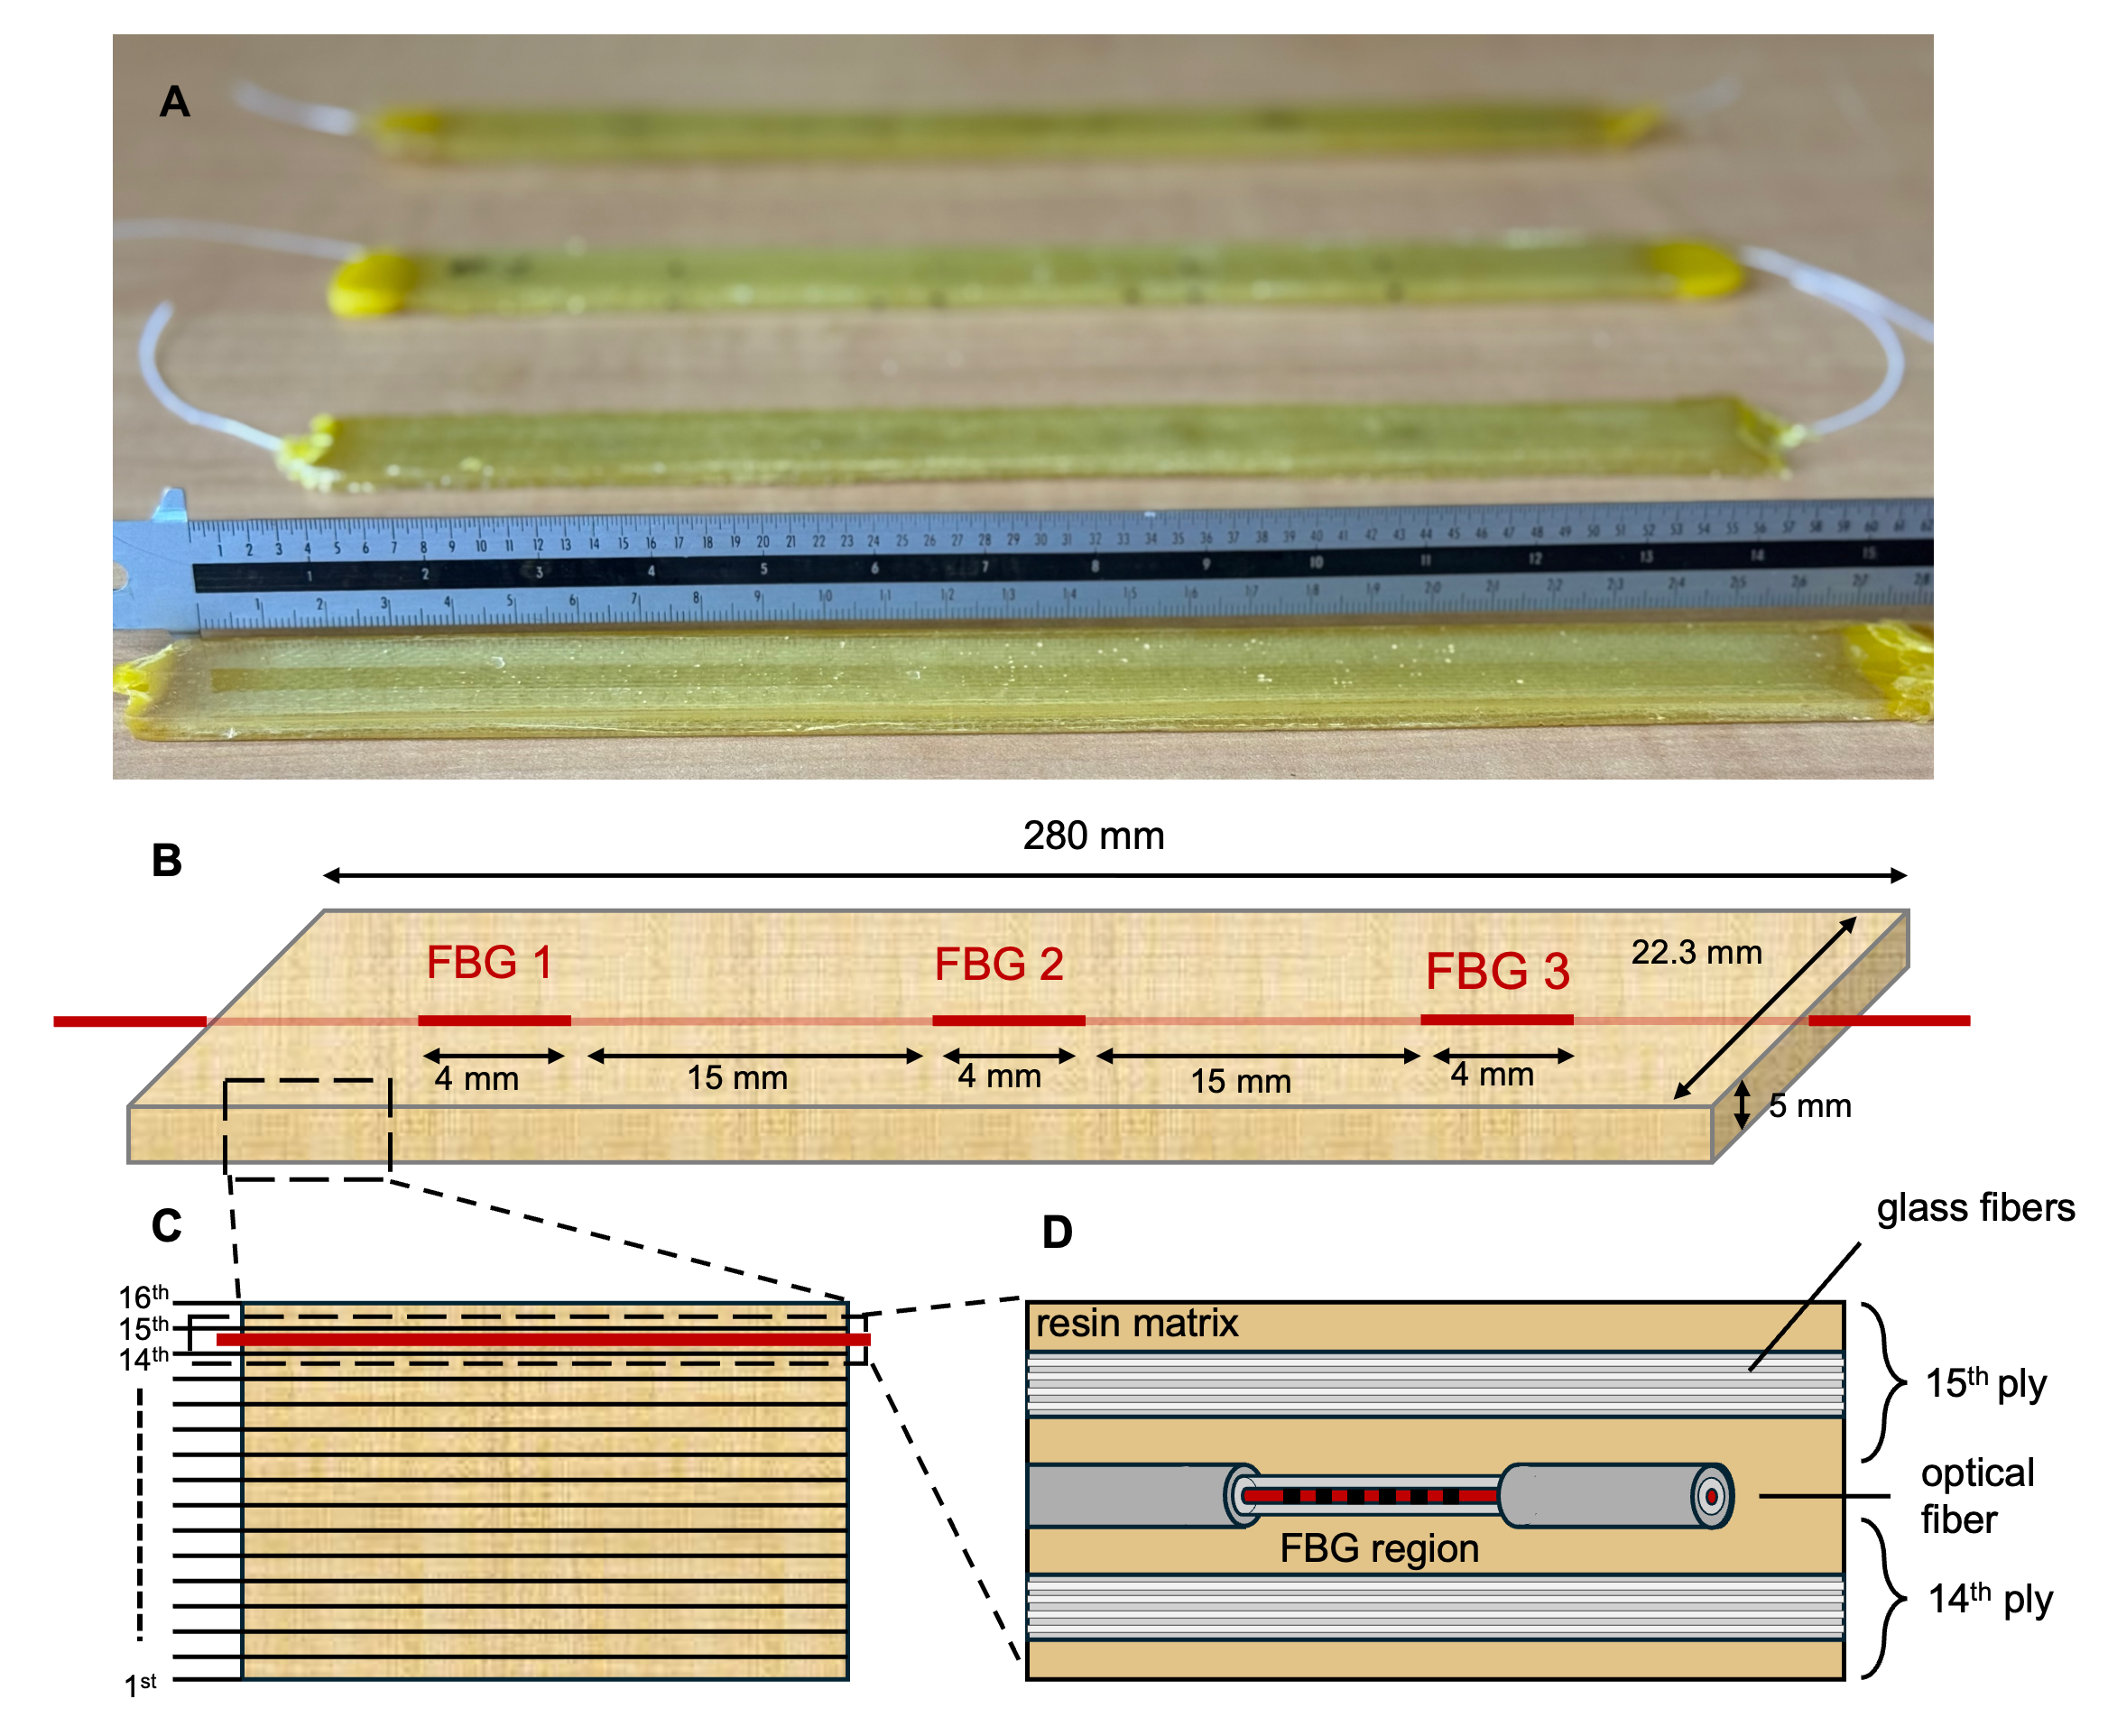
\includegraphics[width=\linewidth]{img/sketch-of-plies-together}
\caption{\textbf{Fabricated composite specimens, specimen geometry, laminate layup, and local sensor embedding.} Panel A shows representative hand laminated glass fiber reinforced polymer specimens used in the three-point bending experiments, with a ruler provided for scale. Panel B shows the specimen geometry, nominal dimensions, and the positions of the three embedded FBGs along the optical fiber. Panel C shows a cross section schematic of the 16-ply laminate, highlighting fiber placement between the 14th and 15th plies near the upper surface. Panel D shows a close view of this interply region, indicating the glass fiber layers, resin matrix, embedded optical fiber, and the FBG sensing region.}
\label{fig:composite_sample}
\end{figure}

\FloatBarrier

\subsection*{Three-point bending experiments}

Mechanical testing was performed with a pneumatic three-point bending system instrumented to measure applied force and crosshead displacement. Each specimen was placed on two supports separated by a prescribed span, and load was applied at midspan. The actuator force was controlled through discrete air pressure settings. For each selected pressure level, ten consecutive loading cycles were applied before moving to the next level. This protocol produced repeated measurements within a given loading block while progressively increasing the loading level on the specimen. During each test, the bending machine recorded force, displacement, and applied pressure, while the embedded FBGs were interrogated in parallel by the BSI-108 FBG interrogator from B-Sens (hereafter referred to as the FBG interrogator). The instrumented bending setup is shown in Figure~\ref{fig:bending_setup}. In the current dataset, support spans of 110, 150, 190, and 230 mm were investigated, and the nominal specimen width was 22.3 mm.

\begin{figure}[htbp]
\centering
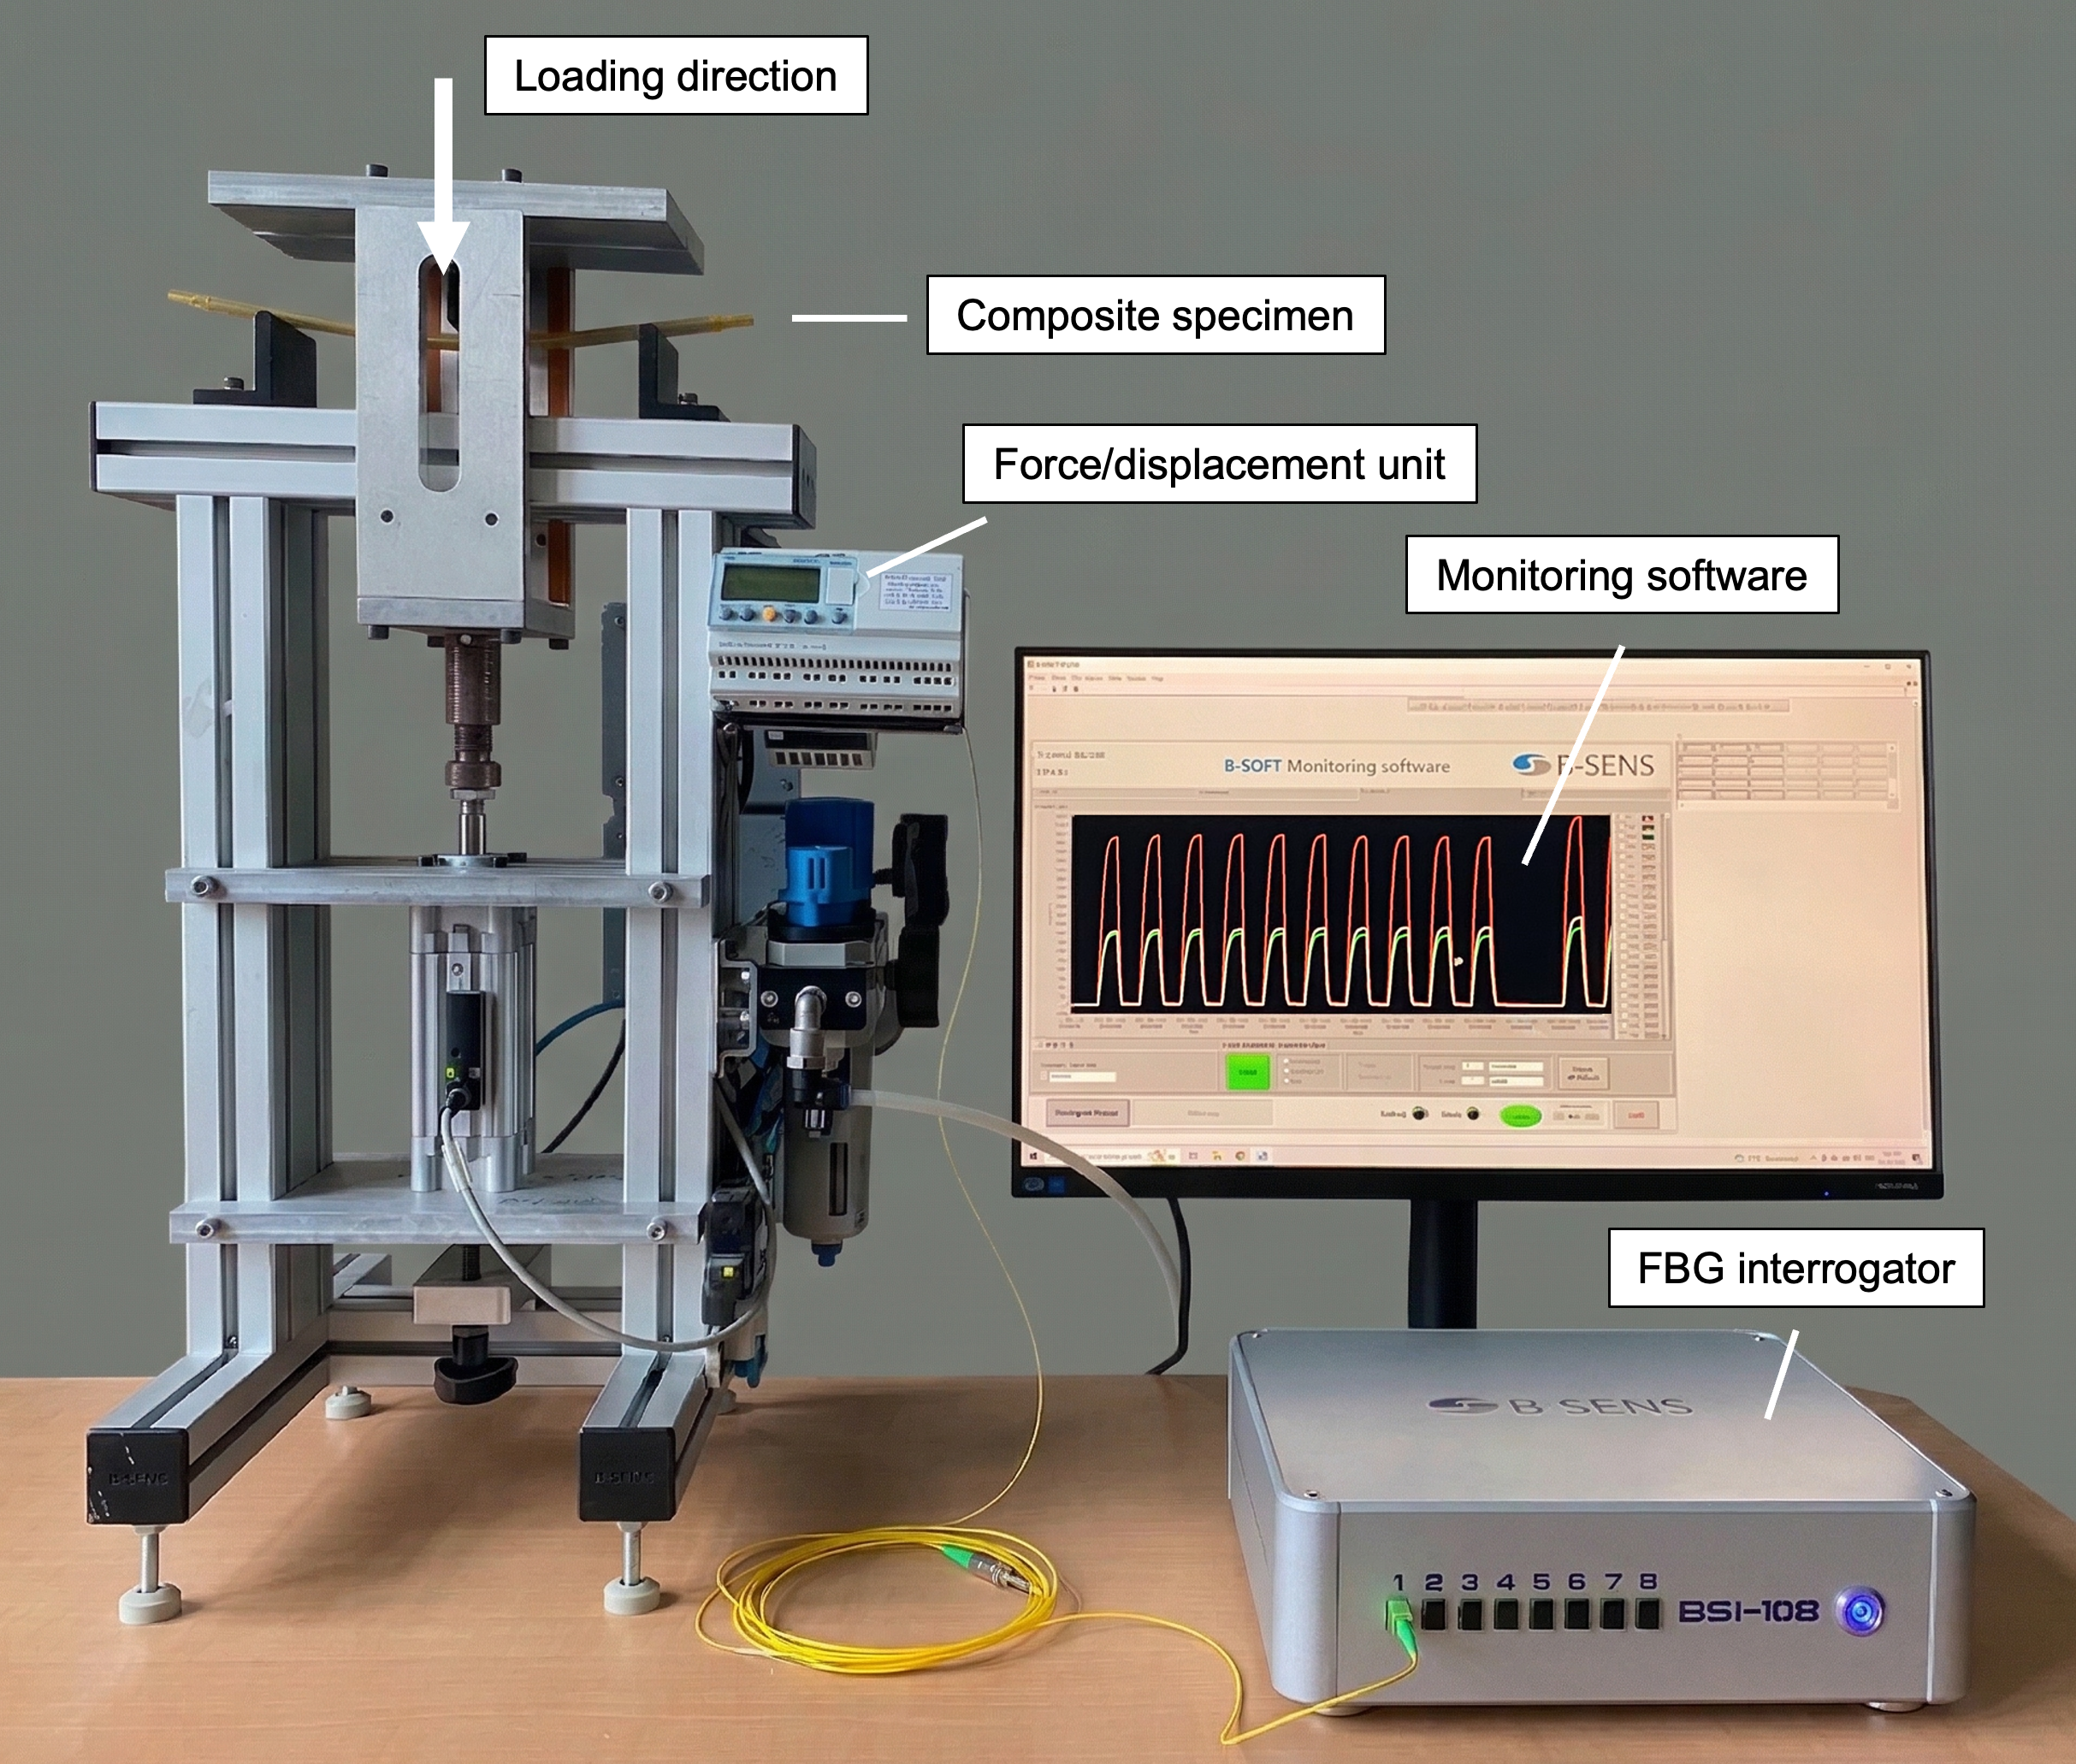
\includegraphics[width=0.7\textwidth, keepaspectratio]{img/experiment-setup-annotated.png}
\caption{\textbf{Three-point bending measurement chain and experimental setup.} Photograph of the instrumented three-point bending system used in the experiments, showing the loading direction, the composite specimen, the force/displacement unit, the monitoring software displayed on the acquisition computer, and the BSI-108 FBG interrogator from B-Sens.}
\label{fig:bending_setup}
\end{figure}

\FloatBarrier

\subsection*{Mechanics based strain interpretation}

The mechanics-informed part of the study is based on the linear elastic response of a slender beam under three-point bending. Similar FBG bending studies have shown that, when embedding is well controlled, the measured wavelength shift can be interpreted consistently with beam theory strain fields in the elastic regime \cite{gabardi2023}. For a simply supported specimen loaded at midspan, the applied force generates a bending moment that produces tension on one side of the beam and compression on the other, while the longitudinal strain vanishes at the neutral axis. An embedded FBG located away from this axis therefore experiences a strain that depends on both the applied load and its position through the thickness. In the present configuration, the maximum bending moment is
\[
M = \frac{F L}{4},
\]
where $F$ is the applied force and $L$ is the support span. According to Euler-Bernoulli beam theory, the longitudinal stress varies linearly with the distance $y$ from the neutral axis \cite{ochsner2021}:
\[
\sigma = \frac{M y}{I},
\]
where $I$ is the second moment of area of the cross section. For the rectangular specimens considered here,
\[
I = \frac{b h^3}{12},
\]
with $b$ the specimen width and $h$ the specimen thickness. Assuming linear elastic behavior before crack initiation, $\varepsilon = \sigma / E$, so the strain at the FBG position becomes
\begin{equation}
\varepsilon = \frac{M y_{\mathrm{FBG}}}{E I} = \frac{3 F L y_{\mathrm{FBG}}}{E b h^3},
\label{eq:euler_bernoulli_strain}
\end{equation}
where $E$ is the effective Young's modulus and $y_{\mathrm{FBG}}$ is the signed distance of the sensor from the neutral axis. This expression provides a simple estimate of the elastic strain expected from an undamaged specimen; deviations between measured and predicted responses therefore motivate the mechanics-informed descriptors used in this work. Before constructing these descriptors, the elastic bending response was examined to verify that beam theory described the behavior before crack initiation. As shown in Figure~\ref{fig:calibration_plots}A, the applied force increased approximately linearly with the measured displacement over the initial loading regime of the calibration specimens. A departure from this linear trend appeared at higher displacement levels, consistent with the onset of nonelastic behavior and supporting the restriction of the mechanics calibration to the regime before crack initiation.

Using the measured wavelength shifts, an FBG strain sensitivity of 1.2 pm/$\mu\varepsilon$ determined from a calibration process, and the Euler-Bernoulli relation in Eq.~\ref{eq:euler_bernoulli_strain}, an effective Young's modulus was estimated from calibration data collected before crack initiation. Figure~\ref{fig:calibration_plots}B shows that the resulting modulus values remained clustered around 18.6 GPa across the investigated force range, with limited dispersion. This supported the use of a single effective modulus of 18.6 GPa for the mechanics-informed analysis, a value consistent with reported elastic moduli for GFRP laminates and woven GFRP composites in the literature \cite{bazli2019,gao2016}. It was then used to compute the elastic strain expected at each loading level and to quantify deviations between measured and expected responses.

\begin{figure}[htbp]
\centering
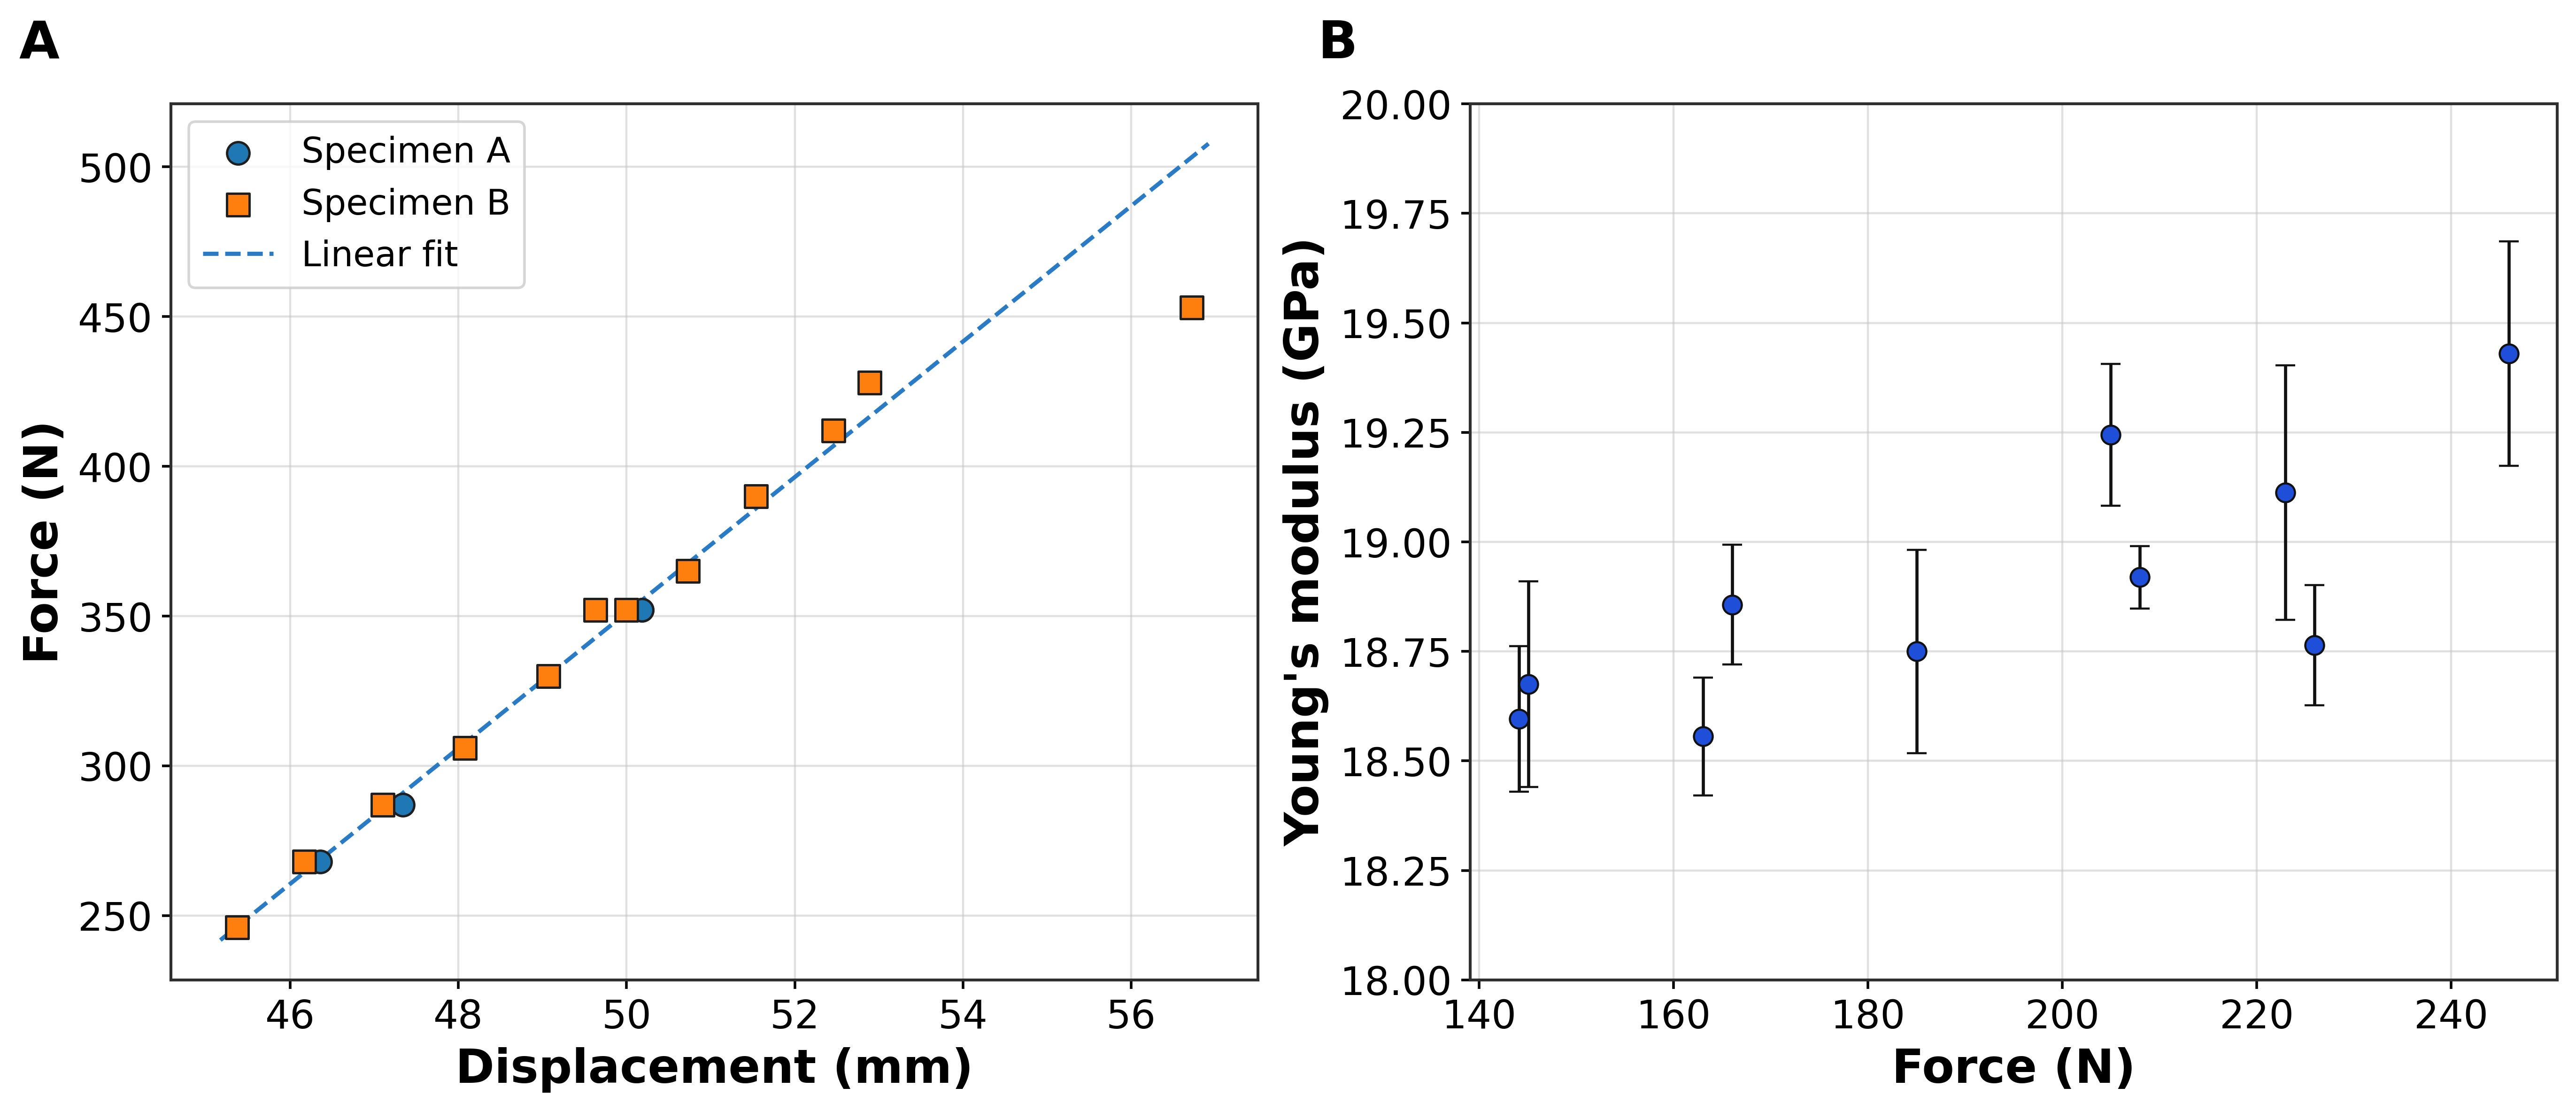
\includegraphics[width=\linewidth]{img/calibration_mechanics_combined}
\caption{\textbf{Calibration of the 16-ply specimens in the elastic regime.} Panel A shows the measured force as a function of displacement for Specimens A and B, together with the fitted linear trend used to identify the initial elastic regime. Panel B shows the effective Young's modulus estimated from calibration measurements before crack initiation using the FBG wavelength shifts and the Euler-Bernoulli bending relation. The limited dispersion across the investigated force range supports the use of a single effective modulus for the mechanics-informed model.}
\label{fig:calibration_plots}
\end{figure}

\FloatBarrier

\subsection*{Data acquisition, peak alignment, and window construction}

The dataset was built from two synchronized sources: raw multiplexed interrogator recordings and experiment-level mechanical metadata. The FBG interrogator tracked the Bragg peak evolution of the active sensor channels over the 1510--1590 nm spectral range with sub-picometer wavelength resolution, while the bending setup recorded force, displacement, applied pressure, support span, and specimen geometry for each loading group. The learning dataset was reconstructed directly from the raw interrogator text files and the associated spreadsheet metadata rather than from pre-aggregated summary tables. This design preserves the waveform shape of each loading response, exposes the full alignment path, and retains the information needed to test whether loading context improves detection.

Each experimental run was segmented into repeated loading responses centered on interrogator peaks. Two alignment strategies were examined: a fully automatic peak search performed directly on the raw interrogator traces, and a hybrid strategy using segment-boundary hints extracted from the aligned experiment records when those hints were available and internally consistent. The hybrid strategy produced the most stable run-level classification results and was therefore used for the main experiments. After segmentation, each retained response was resampled to a fixed-length representation while preserving the synchronized target channel and companion channels from the same multiplexed acquisition. This reconstruction step was central to the study because it converted raw interrogator files into repeatable learning units tied to the mechanical loading history.

The final dataset contained 65 processed runs. For most runs, 120 peak-centered responses were retained, corresponding to 12 loading groups with 10 repetitions per group, although a small number of runs contained fewer usable responses because of incomplete or irregular recordings. Each response was associated with a run identifier, loading-group index, repetition index, sample indices in the original interrogator trace, and the synchronized loading metadata for the corresponding mechanical block. In addition to the raw interrogator channels, the dataset stored aligned loading traces for applied pressure, force, displacement, and an approximate elastic strain target derived from beam theory. This made it possible to derive compact sequence features from the optical response while preserving the synchronized mechanical context.

A window was labeled as crack-associated when it belonged to a loading group annotated as cracked in the experiment spreadsheet used during data acquisition. The label therefore represents a crack-related event state at the loading-group level. The task is formulated as crack-event detection from multiplexed FBG measurements.

Mechanical metadata were aligned to the interrogator windows at the level of repeated loading blocks. Force, displacement, pressure, support span, specimen thickness, and specimen width were assigned to each window through the combination of run identifier and loading-group index. These synchronized quantities were then used to derive the retained loading features, the residualized response terms, and the post hoc physics-consistency filter. Because windows from the same run remained temporally and mechanically correlated, all evaluation protocols were performed at run level rather than by random window splitting.

Figure~\ref{fig:window_mosaic} shows this hierarchy on one sequence. Panel A shows the full interrogator run together with the loading group selected for closer inspection. Panel B zooms into the corresponding 10-window group and highlights windows before crack initiation and crack windows. Panels C and D then show the individual windows used to illustrate the local waveform changes observed across the multiplexed FBG channels before and after crack initiation.

\begin{figure}[htbp]
\centering
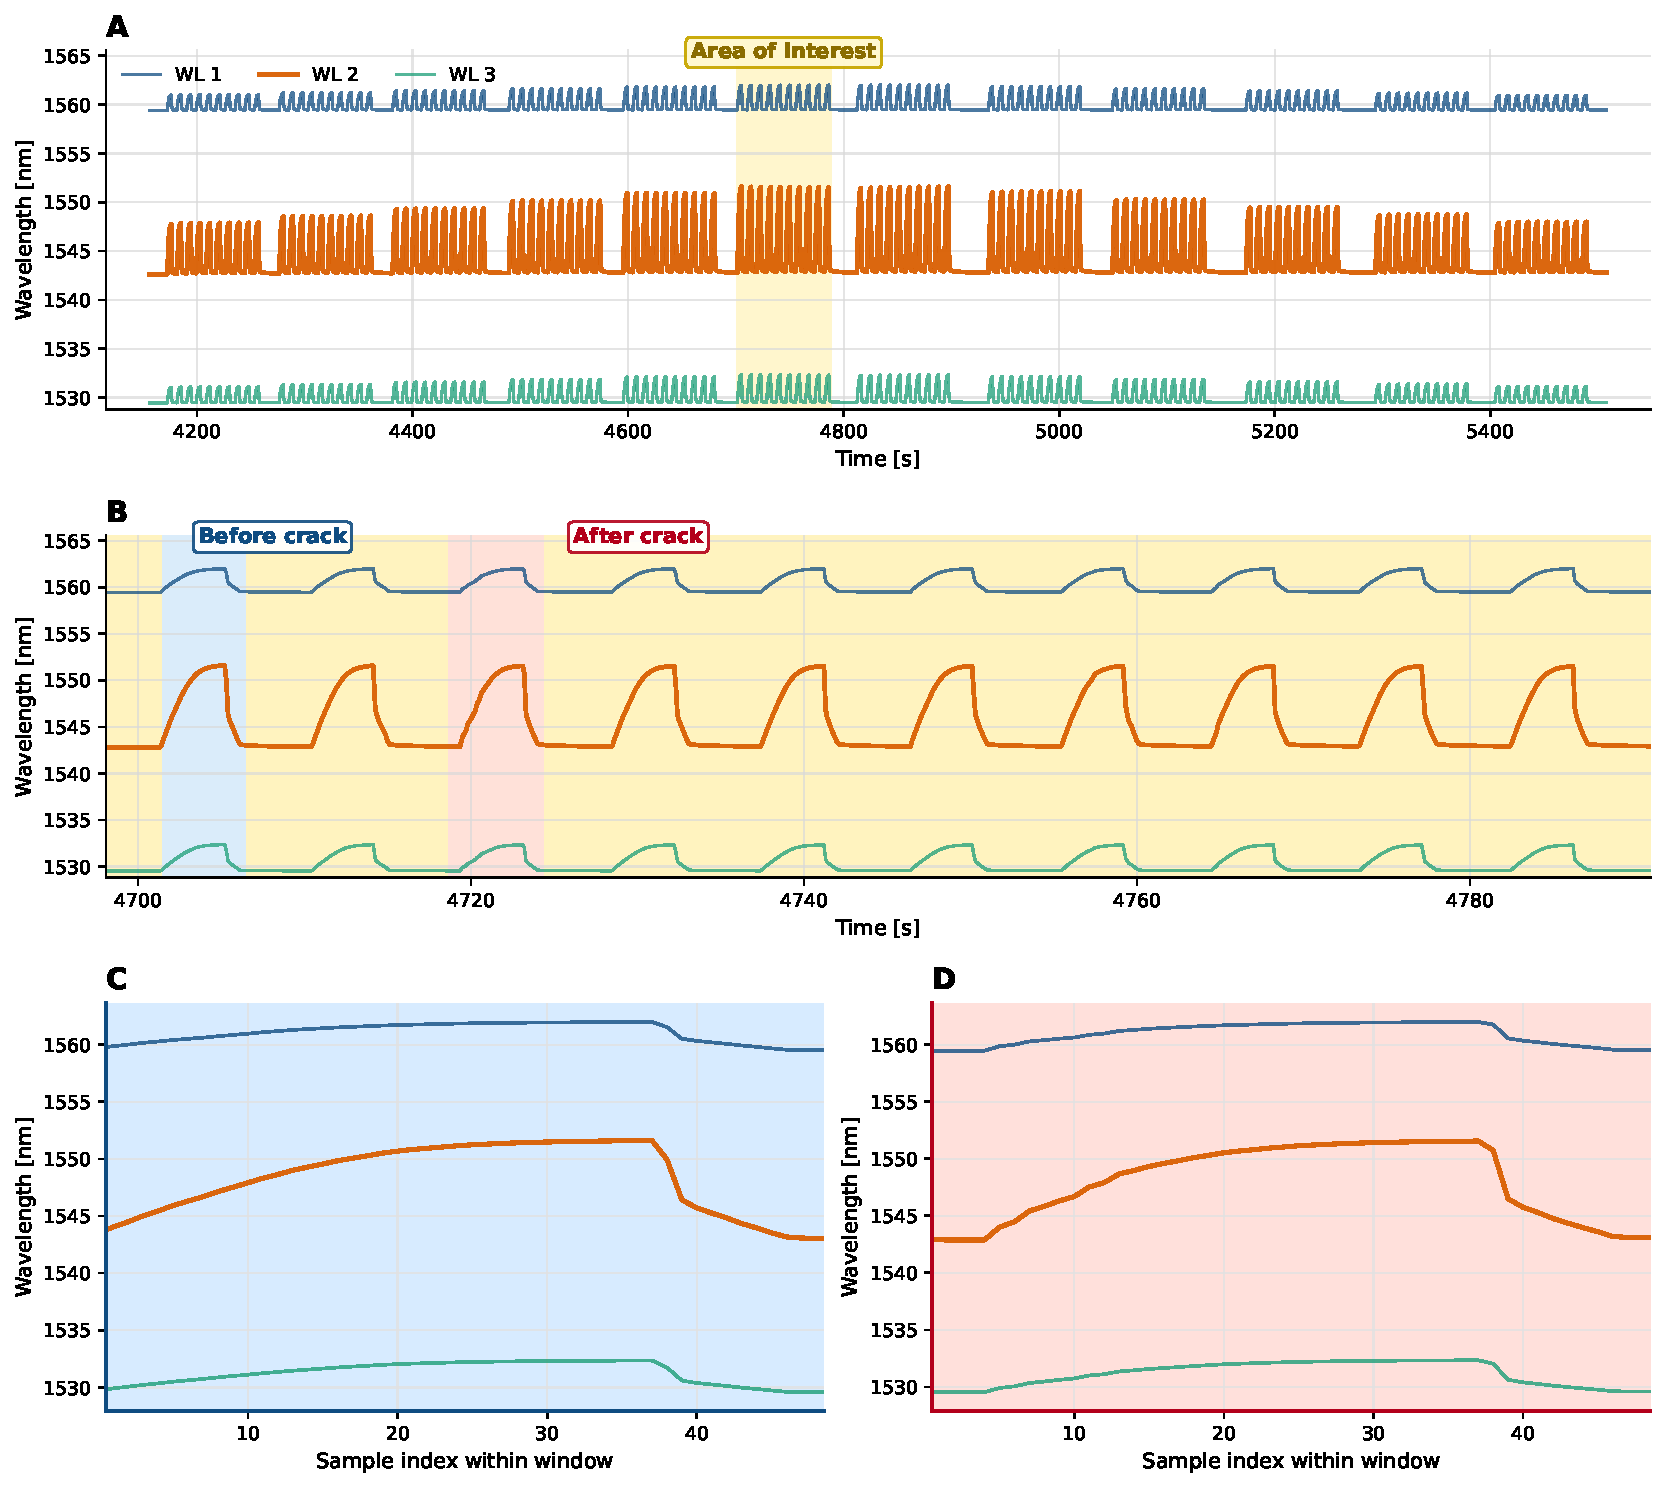
\includegraphics[width=\linewidth]{img/mosaic_time_series_before_after}
\caption{\textbf{Example raw interrogator sequence and window hierarchy used for learning.} Panel A shows the full multiplexed FBG interrogator run, with the selected loading group highlighted. Panel B shows the corresponding 10-window group on a shorter time scale, with windows before crack initiation and crack windows highlighted. Panels C and D show the individual windows before and after crack initiation, respectively, for the target FBG channel together with its two companion channels. This view shows how the raw interrogator signal was organized into loading group context and fixed length windows before feature extraction and learning.}
\label{fig:window_mosaic}
\end{figure}

\FloatBarrier

\subsection*{Sequence representation and synchronized loading features}

The selected paper baseline represents each repeated peak-centered response by a compact feature vector instead of the full interrogator waveform. This representation was retained because it produced the most reproducible strict run-level result among the evaluated alternatives. Nine features were used in the final model: the median wavelength of the target channel, the within-response standard deviation of that wavelength, a run-baseline-residualized target-channel wavelength shift, synchronized force, synchronized crosshead displacement, applied air pressure, the first-difference of the residualized wavelength shift across consecutive responses, the first-difference of the displacement signal across consecutive responses, and a binary flag indicating the reduced-size specimen subgroup identified in the source filenames. These features are summarized in Table~\ref{tab:input_summary}.

\begin{table}[htbp]
\centering
\caption{\textbf{Nine input features used by the selected sequence CNN.} All features were computed for each retained peak-centered response after alignment with the experimental loading records.}
\label{tab:input_summary}
\small
\begin{tabular}{p{0.22\linewidth}p{0.70\linewidth}}
\hline
Feature & Description \\
\hline
\texttt{wl2\_median} & Median wavelength of the target FBG channel within the retained peak-centered response \\
\texttt{wl2\_std} & Standard deviation of the target-channel wavelength within the retained response \\
\texttt{delta\_wl\_ch2} & Target-channel wavelength shift residualized relative to the run baseline \\
\texttt{force\_N} & Synchronized applied force for the aligned loading block \\
\texttt{displacement\_mm} & Synchronized crosshead displacement for the aligned loading block \\
\texttt{air\_pressure\_bar} & Pneumatic loading pressure associated with the aligned loading block \\
\texttt{delta\_wl\_rate} & First-difference of \texttt{delta\_wl\_ch2} across consecutive retained responses within the same run \\
\texttt{delta\_disp\_rate} & First-difference of displacement across consecutive retained responses within the same run \\
\texttt{is\_small\_sample} & Binary indicator for the reduced-size specimen subgroup encoded in the source filenames \\
\hline
\end{tabular}
\end{table}

\FloatBarrier

Each learning sample comprised 30 consecutive retained responses from the same run, with stride 1. The label attached to each 30-response sequence was the maximum of the crack-event labels already present within that sequence and the label observed at a prediction horizon of 5 responses beyond the sequence end. This rule preserved sensitivity to transitions that emerged near the end of a local response history while keeping the sequence definition fixed across runs. Feature normalization was fitted on the training split only within each validation fold. Samples with invalid indices or missing synchronized values were excluded during dataset construction, and no imputation was used.

\subsection*{Selected simple sequence CNN}

The retained classifier is a compact one-dimensional CNN operating on a $30\times9$ input array, where the 30 rows correspond to ordered retained responses and the 9 columns correspond to the synchronized feature set described above. During inference, the feature dimension is treated as the channel dimension and the sequence order is treated as the temporal dimension. The network uses three temporal convolution layers with 32, 64, and 128 channels, all with kernel size 12 and padding 6, each followed by a rectified linear unit activation. Adaptive average pooling then compresses the temporal representation to a single 128-dimensional embedding, which is passed to a classifier head composed of a 64-unit fully connected layer, rectified linear unit activation, dropout of 0.2, and a final linear output layer producing one crack-event logit.

This architecture was selected because it keeps the modeling pipeline simple while still allowing the network to learn short-range temporal motifs across consecutive loading responses. Figure~\ref{fig:physics_architecture} summarizes the retained pipeline from peak alignment to run-level decision.

\begin{figure}[htbp]
\centering
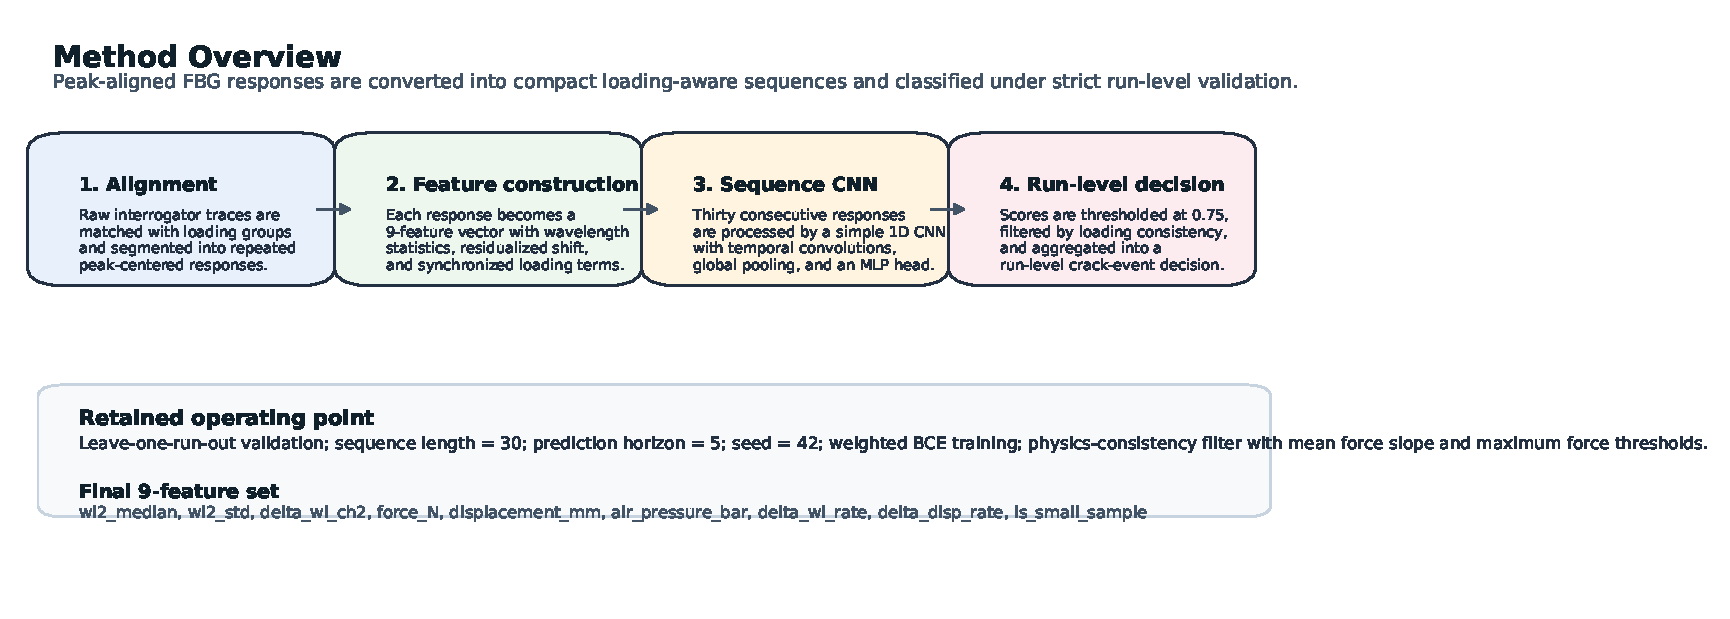
\includegraphics[width=\linewidth]{img/simple_sequence_cnn_pipeline}
\caption{\textbf{Selected sequence CNN pipeline used for the main manuscript result.} Raw interrogator recordings were first aligned with the experiment records and segmented into repeated peak-centered responses. Each response was then converted into a nine-feature vector combining target-channel wavelength statistics, residualized wavelength shift, synchronized loading quantities, first-difference terms, and a specimen-size flag. Sequences of 30 consecutive responses were processed by a simple one-dimensional CNN, thresholded at 0.75, filtered by loading-consistency rules, and finally aggregated into run-level crack-event decisions.}
\label{fig:physics_architecture}
\end{figure}

\FloatBarrier

\subsection*{Training, model selection, and evaluation}

This study uses run-level evaluation because neighboring retained responses from the same run are highly correlated. The main protocol therefore uses leave-one-run-out validation, implemented as leave-one-group-out cross-validation with the run identifier as grouping variable. In this setting, each held-out fold corresponds to an unseen experimental run, and run-level predictions are obtained by aggregating the sequence predictions within that run.

The selected operating point used the reconstructed aligned dataset generated from the raw interrogator files together with the retained segment-boundary hints from the merged experiment records. Training used weighted binary cross-entropy to account for class imbalance, a fixed random seed of 42, batch size 128, Adam optimization with learning rate $10^{-3}$ and weight decay $10^{-4}$, a maximum of 8 epochs, and early stopping with patience 3 on the inner validation split. Mixup and reduced feature-set ablations were explored during development, but they were not retained because they did not improve the strict run-level $F_1$ of the final operating point.

At the end of each fold, validation probabilities were used to select the decision threshold. The retained main result uses a fixed threshold of 0.75 together with a post hoc physics-consistency filter derived from the aligned loading trace. This filter suppresses predicted positives when the mean force slope across the 30-response sequence is below $-0.1$ or when the maximum force in that sequence is below 100 N. The purpose of the filter is to reject detections that are inconsistent with the expected monotonic loading regime of the bending protocol.

Experiment-level precision, recall, $F_1$, and balanced accuracy are reported first because they reflect generalization across independent runs. Pooled window-level metrics and ROC-AUC are reported as complementary information. Grouped five-fold evaluation is retained only as a secondary comparison and is not used as the primary claim.

\section*{Results}

\subsection*{Offline crack-event detection performance}

The main evaluation was performed with strict leave-one-run-out validation on the reconstructed aligned dataset. The selected operating point used the simple sequence CNN described in Methodology, a fixed threshold of 0.75, and the post hoc physics-consistency filter. Table~\ref{tab:overall_performance} reports experiment-level metrics first, followed by the corresponding pooled window-level metrics for context.

\begin{table}[htbp]
\centering
\caption{\textbf{Strict run-level results for the selected CNN operating points.} All rows use the same leave-one-run-out protocol, sequence length of 30 windows, prediction horizon of 5 windows, and grouped predictions at run level. The selected paper result is the fixed-threshold model with the physics-consistency filter at threshold 0.75.}
\label{tab:overall_performance}
\small
\begin{tabular}{p{0.37\linewidth}cccc}
\hline
Operating point & Precision & Recall & $F_1$ & Bal. accuracy \\
\hline
Strict LOOCV baseline (no physics filter) & 0.600 & 0.600 & 0.600 & 0.739 \\
Strict LOOCV + physics filter at threshold 0.75 & 0.833 & 0.667 & 0.741 & 0.813 \\
Strict LOOCV + physics filter at threshold 0.80 & 0.800 & 0.533 & 0.640 & 0.746 \\
\hline
\end{tabular}
\end{table}

\FloatBarrier

\subsection*{Effect of thresholding and the physics-consistency filter}

The strict leave-one-run-out baseline without the physics-consistency filter reached experiment-level precision of 0.600, recall of 0.600, and $F_1$ of 0.600. Applying the filter and selecting a threshold of 0.75 improved precision to 0.833, recall to 0.667, and $F_1$ to 0.741. At run level, this corresponds to a reduction in false-positive runs from 6 to 2 and an increase in true-positive runs from 9 to 10. The same operating point gave a balanced accuracy of 0.813.

The threshold sweep showed that this gain was not obtained by simply lowering the decision threshold. Below 0.75, recall remained 0.667 but precision dropped steadily, falling to 0.455 at threshold 0.50. Above 0.75, precision remained high but recall fell to 0.533 at threshold 0.80 and to 0.400 at thresholds 0.85 and above. Within the tested range, threshold 0.75 therefore provided the best experiment-level $F_1$ while preserving the highest recall achieved by the filtered model.

At window level, the selected filtered operating point produced precision of 0.768, recall of 0.414, $F_1$ of 0.538, balanced accuracy of 0.697, and ROC-AUC of 0.719. These pooled window metrics are lower than the experiment-level values because many neighboring windows within a run remain correlated and because the run-level aggregation emphasizes whether a specimen-level test is flagged correctly rather than how many individual windows are classified as positive.

\begin{figure}[htbp]
\centering

\includegraphics[width=\linewidth]{img/strict_loocv_results_summary}
\caption{\textbf{Run-level behavior of the selected strict operating point.} Panel A shows the experiment-level precision, recall, and $F_1$ obtained after application of the physics-consistency filter across the tested decision thresholds. The selected threshold of 0.75 maximized experiment-level $F_1$ while preserving the highest recall achieved by the filtered model. Panel B compares the run-level error profile of the unfiltered strict baseline with the selected filtered operating point, showing the increase in true-positive runs and the reduction in false-positive runs.}
\label{fig:strict_results_summary}
\end{figure}

\FloatBarrier

\subsection*{Merge strategy and secondary comparisons}

The best reproducible result was obtained from the reconstructed raw dataset when peak-centered windows were aligned with the segment-boundary hints inherited from the merged experiment records. A fully automatic raw peak search produced a less stable dataset and lower strict run-level performance. This indicates that data alignment remains a major determinant of final score and should be considered part of the method rather than a preprocessing detail.

As a secondary benchmark, grouped five-fold evaluation without the physics filter produced experiment-level precision of 0.875, recall of 0.467, and $F_1$ of 0.609. This score is lower than the selected strict operating point and is not used as the primary claim. The leave-one-run-out result remains the main benchmark because it preserves specimen separation explicitly.

\section*{Discussion}

These results show that crack-event detection is feasible from short peak-aligned windows of multiplexed FBG interrogator data when synchronized loading metadata are incorporated into the pipeline. The selected strict operating point reached experiment-level precision of 0.833, recall of 0.667, and $F_1$ of 0.741. For the present dataset, the strongest improvement came from combining a simple CNN with alignment-aware preprocessing and a mechanics-motivated consistency filter rather than from increasing architectural complexity. This is an important result because it shows that useful specimen-level damage information can be extracted from compact multiplexed FBG measurements with a method that remains interpretable and reproducible.

The results also show that metric choice matters. Pooled window scores alone understate and sometimes distort specimen-level behavior because adjacent windows from the same run remain highly dependent. Reporting experiment-level precision, recall, $F_1$, and balanced accuracy first is therefore more appropriate for this problem than relying on headline window-level scores. This evaluation choice strengthens the practical value of the study because it tests whether the model generalizes across independent runs rather than across nearly repeated windows from the same run.

Mechanics plays a practical role in the present study by structuring the detection pipeline around synchronized loading information. Force and displacement traces, residualized response features, and a post hoc filter based on monotonic loading consistency provide structural constraints that reduce implausible detections and improve run-level performance. This supports the broader idea that structural priors can strengthen learning from sparse optical measurements when the sensing configuration does not provide rich spatial information.

Recall remains an important area for improvement. The selected operating point reached a recall of 0.667 while preserving a clear gain in precision and overall experiment-level $F_1$ relative to the unfiltered baseline. The threshold sweep also showed that further increases in recall on the current dataset were accompanied by a marked loss of precision, which suggests that the present bottleneck is tied not only to threshold selection or training duration, but also to label granularity, sample count, and alignment quality.

Another limitation is the supervision itself. Labels were inherited from loading-group annotations in the experiment records rather than from an independent spatial crack-mapping procedure. The method should therefore be interpreted as a crack-event detector at loading-group level, not as a validated crack-localization system. In addition, the best result depended on a specific alignment strategy that reused reliable boundary hints from the merged records, which underscores the sensitivity of the pipeline to data reconstruction choices.

Overall, the study supports the use of compact CNN-based models for crack-event detection from multiplexed FBG measurements, provided that claims remain aligned with the available supervision and the evaluation protocol is kept strict. The work establishes a reproducible baseline, clarifies the importance of alignment in this sensing setting, and shows how simple mechanics-guided constraints can improve detection quality. The most credible next improvements are better aligned labels, more independent runs, and stronger physically meaningful synchronization between interrogator traces and mechanical loading records.

\section*{Data availability}

All data are available upon reasonable request to the corresponding author.

\section*{Code availability}

The code used in this study is available from the corresponding author upon reasonable request.

\bibliography{sample}

\section*{Funding}

The authors acknowledge financial support from Walloon Region of Belgium through the Interreg VI France-Wallonie-Vlaanderen program co-funded by the European Union, under SALOME project (No. 0100240). This work was also supported by WEL Research Institute and the Fonds de la Recherche Scientifique (F.R.S.--FNRS).

\section*{Acknowledgments}

The authors thank Mariel David for her assistance during the manufacturing of the composite specimens. The authors also thank Damien Kinet from B-SENS for his assistance with the operation of the three-point bending system.


\section*{Author contributions statement}

A.U. analyzed the data, applied the machine learning algorithm, and contributed to writing the manuscript. A.G. supervised the machine learning aspects of the study. E.N. and T.T. cured the composite specimens and conducted the three-point bending experiments. K.Y. supervised the FBG-related aspects of the study. K.C. assisted with FBG inscription and curing of the composite specimens. C.C. supervised the FBG-related aspects of the study and wrote the manuscript.

\section*{Additional information}

Competing interests: The authors declare no competing interests.

\end{document}
